\documentclass[journal]{ieee_style}

\usepackage{amsfonts}
\usepackage{minted}
\usepackage{graphicx}
\usepackage{amssymb}
\usepackage{amsmath}
\usepackage{latexsym}
\usepackage{caption}
\usepackage{mathtools}
\usepackage{url}
\usepackage{array}
\usepackage{hyperref}


% correct bad hyphenation here
\hyphenation{op-tical net-works semi-conduc-tor}


\begin{document}
\title{Power-Based Side-Channel Attack for AES Key Extraction on a ATMega328 controller}

\author{Utsav Banerjee,
        Lisa Ho,
        and Skanda Koppula% <-this % stops a space
\thanks{All authors are with the Department
of Electrical and Computer Engineering, Massachusetts Institute of Technology, Cambridge,
MA, 02139 USA}% <-this % stops a space
\thanks{To contact the authors: \texttt{utsav@mit.edu}, \texttt{lisaho@mit.edu}, and \texttt{skandak@mit.edu}}% <-this % stops a space
\thanks{Manuscript completed for 6.858 Computer Systems Security; completed on December 5, 2015}}

\markboth{6.858 Final Project Report - Fall 2015}%
{Power-Based Side-Channel Attack for AES Key Extraction on the ATMega328 controller}
\maketitle

\begin{abstract}
    We demonstrate extraction of a private-key from Flash program memory on the ATMega328 microcontroller (the controller used on the popular Arduino Genuino/Uno board). We loaded a standard AVR-architecture AES implementation onto the chip and ran this implementation to encrypt 500 randomly chosen plaintexts. By carefully measuring the chips power consumption, we were able to correlate the consumed power with the input plaintexts and key values that might be used to encrypt each AES block, and back-derive the hard-coded key used for encryption. We describe here our test infrastructure for automated power trace collection, an overview of our correlation attack, sanitization of the traces and interesting stumbling blocks encountered during data collection and analysis, and the results of our attack.
\end{abstract}

\begin{IEEEkeywords}
AES, side-channel, power consumption, ATMega328, Correlation Power Analysis
\end{IEEEkeywords}

\section{Introduction}
Recent concerns about data privacy has brought attention to the necessity of encryption algorithms. One of the more popular symmetric-key algorithms, Advanced Encryption Standard (AES), has been the U.S. government standard since 2002 (ISO/IEC 18033-3), and is used in a multitude of applications: SSL/TLS protocols \cite{ssl}, Kerberos \cite{kerberos}, and demonstrably secure embedded devices \cite{embedded}. This last application in particular, embedded devices, has seen much growth in recent years, given the advantages of computation on smaller embedded devices: low power, lower system latency, and generally smaller device size.

Small hardware implementations, however, are notoriously vulnerable to a range of side-channel attacks \cite{smalldevice}. Timing, electromagnetic radiation, and power consumption are just three commonly exploited vectors used to leak information about ongoing computations and data on the chip. Knowing that a device architecture is amiable to side-channel exploitation is useful in deciding whether to execute unprotected sensitive computations or store data on devices with similar memory and processor characteristics.

We aim to demonstrate a reasonably realistic side-channel attack on AES on one such embedded device: the ATMega328 microcontroller produced by Atmel. The ATMega328 is the basis for the widely popular development board, Arduino Uno \footnote{Other models of the Arduino, such as the Arduino Mega and Arduino Genuino Micro use ATMega chips as well, that have a similar architecture to the ATMega328. It is possible that this attack could be adapted to those chips as well.}

In section two, we review for the read the theoretical ideas underpinning our attack. In section three, we describe our implementations our hardware setup, power measurement infrastructure, correlation methodologies, instructive problems that we encountered, and overview the structure of our source code. In section four, we describe quantitatively describe the results of our attack.

\section{Preliminaries}
\subsection{Controller Specifications}
The ATMega328 family of chips is an 8-bit microcontroller series with 32 KB of NAND-type flash and 2KB of SRAM. The controller runs off a 16 MHz external clock on the Arduino board. Typical power consumption of the chip ranges from 7 to 12V, with a 20mA current draw, depending on the peripheral and I/O pin usage \cite{atmeldatasheet}. Out attack exploits the NAND-type flash memory architecture that consumes marginally more power when accessing addresses that store value-zero (discharge) bits \footnote{In a highly simplified power consumption model, NAND-flash charges a central power line connected to a series of memory cells. Depending on the value stored in the accessed memory cell, the line is discharged or not. Thus, line requires data-dependent recharging.} \cite{nandflash}.

The encryption program running on our ATMega328, \texttt{AESLib}, uses an Arduino-specific port of the \texttt{avr-crypto-lib} by Davy Landman and Bochum Hackerspace \cite{AESLib} \cite{daslabor}. \texttt{AESLib} is one of the more widely-used AES implementations for Arduino, and includes support for ECB and CBC-modes of AES. Our team decided that ECB-mode would be more amiable to a power correlation attack, and correspondingly chose to exploit the library's AES-ECB implementation. We discuss ECB in further depth in section 3.D.

\subsection{Correlation Power Analysis}
% Briefly explain how CPA works
% sbox, AES is a block cipher that encrypts blocks of plaintext in a number 
Correlation Power Analysis (CPA) is a type of side channel attack that relies on power consumption information. On a high level, CPA attempts to correlate observed power consumption with expected power consumption. To a greater extent than more basic forms of power analysis such as Simple Power Analysis, CPA attacks are able to extract secret keys from noisy data. This requires collecting the power consumption of a device performing encryption over many different plaintexts with the same key. We can then build a power model that contains the expected power consumption of the device performing a particular operation during encryption over the given plaintexts with every possible key. 

In our case, we used CPA against AES encryption. There are several operations during AES that can be good candidates to model power consumption for depending on the hardware implementation. Attacks tend to model power from the first round of AES because it is most clear in this round which bytes of plaintext and key are getting combined. Power analysis tends to target the XOR operation in the \texttt{AddRoundKey} or the SBOX substitution during the \texttt{SubBytes} operation, since these can consume predictable amounts of power. Different implementations use different estimates to correlate power consumption with, most commonly the Hamming Weight of the operation result or the Hamming Distance of the input and output of the operation. These may be correlated with the amount of power consumed because reading a "0" or "1" from memory may require a different amount of power.
 
Using CPA against AES requires collecting the amount of power consumed over hundreds of plaintexts. We then calculate the expected power consumption for each of these plaintexts with every possible key. Trying every possible key with AES is possible because a different byte of the key is used for every byte of the plaintext. This reduces our search space to $2^8$ possibilities for each key byte, which allows us to build a power model that takes every one of these $2^8$ key byte possibilities into account for each byte. 

After building a power hypothesis consisting of the amount of power consumed for each possible plaintext with every possible key byte, we can calculate the correlation coefficients between these expected amounts of power and the amount of power observed during encryption. One advantage of CPA is that we don't need to know exactly when during encryption our targeted operation occurs; we can calculate the correlation coefficient between the power hypothesis and the power trace (collected power consumption over time) at each point of the trace. We then take the key byte that gives us the maximum correlation coefficient as our best guess key byte. Repeating this process 16 times gives us best guesses for all 16 bytes of the key.


\section{Protocols and Procedure}
\subsection{Data Collection Infrastructure}
A central piece of our work was developing the serial-connection based data collection framework to feed plaintexts for encryption to the Arduino, and read the resulting power trace from the oscilloscope. An outline is given in Figure 1.

\begin{figure}[!t]
\centering
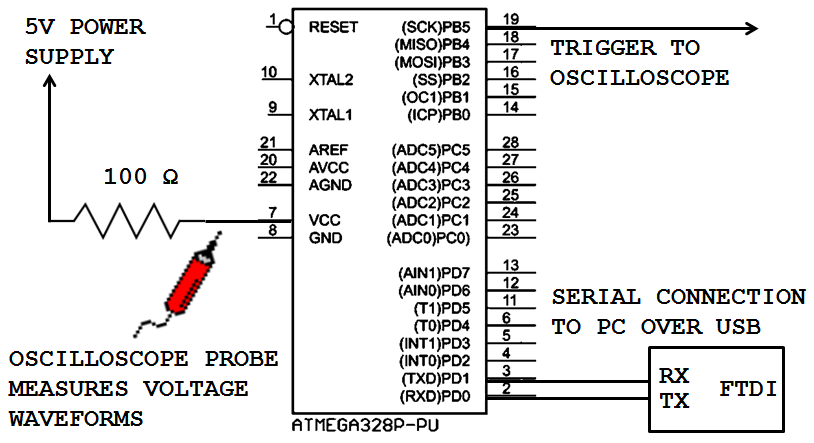
\includegraphics[width=2.5in]{setup}
\caption{The oscilloscope probes voltages on the chip's power line, starting automated power trace on a trigger that signals the start of AES}
\label{fig_sim}
\end{figure}

We needed a subset of the power trace that correlated strongly with the input plaintext and key. Specifically, we were interested in finding the portion of the trace that corresponded to the \texttt{xor(plaintext,key)} operation, and the the SBOX permutation taken over the \texttt{xor} result. In order to automate slicing to this part of the trace, we modified the \texttt{AESLib} SBOX assembly code to insert a flag a memory-mapped register that pulled up pin 13. Our oscilloscope triggered on this output, and automatically captured the part of the trace immediately after the pin 13 rising edge. 

Central to our collection was a Tektronix 5054B computing oscilloscope that collected samples at 4GHz with internal memory bank of at most 16 million points. The sampling rate limited the resolution of traces that we were able to capture; we originally thought this physical cap on data quality was causing correlation issues we ran into, until we discovered arbitrary DC shifts in the traces. We discuss this challenge in more detail in Section 3.C. We used the oscilloscope's GPIB query interface to automate configuration and downloading of traces.

In the final iteration of our system, we have a orchestrating computer $C$ send plaintexts to the Arduino for encryption every 2 seconds over the Arduino's serial port. The pin 13 trigger resulting in a oscilloscope trace capture, which was sent back to $C$. 

More recently, we have been attempting to use the Tektronix $Fast Frames$ feature to take capture batches of 2,500-point traces at once, and use one memory-read, GPIB-write operation to transfer these traces to the computer. This would allow us much faster trace measurement, which is currently bottlenecked by the GPIB-write operation. As we will discuss in Section 4, the number of key bytes we can recover is directly correlated with the number of plaintexts we can capture and average.

Photos of our collection framework can be found at \texttt{\url{https://www.dropbox.com/sh/usialgelvfqlsdr/AACvqOHKEWoumWNYi2WRIebCa?dl=0}}. Of perhaps small interest is the grounded aluminum box encapsulating the ATMega328 setup, which reduced the EM noise and interference which we noticed in our power traces.

\subsection{Implementation of CPA and Power Model}

When we were first deciding what operation to model, we examined AESLib to try to determine what which AES steps might be best to estimate the power consumption for. The XOR operation from the \texttt{AddRoundKey} step consisted of two operations, a load and an XOR: 1) \texttt{ld r0, X+} and \texttt{eor param, r0} where \texttt{param} was a byte of the key and \texttt{X+} was a byte of the plaintext. The SBOX operation from the \texttt{SubBytes} step consisted of a move and load program memory instruction: 1) \texttt{mov r30, ST00}, 2) \texttt{lpm ST00, Z}. We hypothesized that reading from memory might require different amounts of power depending on whether we were reading a ``0'' or a ``1''. We first chose to try to model the power consumed during the SBOX operation, since its nonlinearity would make for clearer key results. However, when we built a power model based on the SBOX operation and then tried to correlate it to our first set of traces, we found no useful correlation. It later became clear that this was a problem with our data rather than our power model (as outlined in III.C). At the time, however, we were concerned that maybe the power consumed by the Arduino was for some reason not proportional to the SBOX output. 

To verify that the results of the SBOX and XOR operations were actually correlated by the amount of power the Arduino consumed, we experimented with modelling the expected power consumption from both operations atomically. We examined the power consumption of just the AVR assembly operations corresponding to these steps on the Arduino. We were unable to easily make out any difference in power consumption between when the result of the SBOX operation was all ``0''s or all ``1''s, but we were able to easily see a diffference in power consumption between when the result of the XOR operation was all ``0''s or all ``1'' (see figure below).

\begin{figure}[!t]
\centering
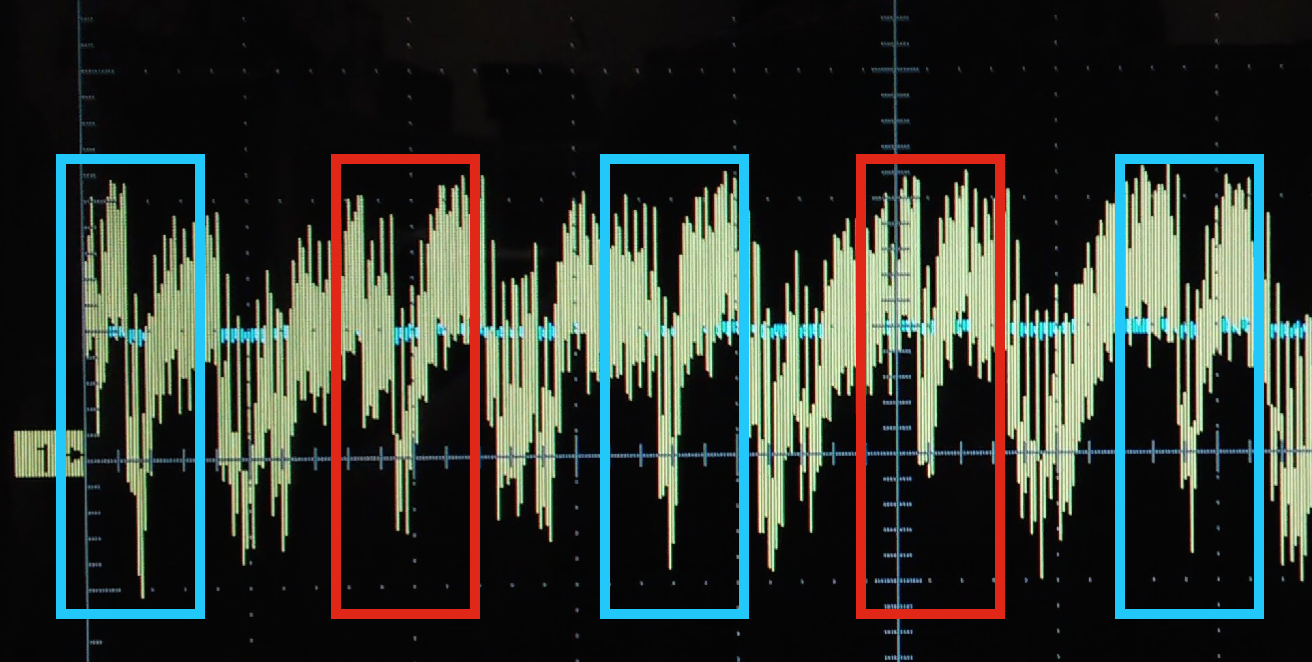
\includegraphics[width=2.5in]{XOR_PC}
\caption{XOR operations alternated between results of all "0"s and all "1"s. The power consumption was noticeably different depending on the Hamming Weight of the result.}
\label{fig_sim}
\end{figure}

Based on these results, we chose to move forward by correlating the power consumption with the Hamming Weight of the XOR result. After collecting more reliable traces (as explained in III.C), we reran CPA using this metric and were able to recover many of the key bytes. However, we ran into a symmetry issue. Each key byte had an equal correlation with the power consumption as its complement with respect to 255 (e.g. key byte candidates such as 1 and 255 or 3 and 252 showed the same correlation) when we used the result of the XOR. When the plaintext byte was \texttt{x} and \texttt{255-x}, we got XOR outputs \texttt{y} and  \texttt{~y}, respectively. These opposites were equally correlated (or anti-correlated) with our power model. Taking this into account, we were able to correctly guess $\frac{11}{15}$ key bytes down to the correct key byte \texttt{k} or \texttt{255-k}. 

This symmetry from the XOR output meant we wouldn't be able to recover the correct key without applying brute force guessing after running CPA. Using the output of the SBOX for the power model would have the advantage of avoiding this symmetry, giving us one correct key. After getting more reliable traces, we retried CPA with a power model employing the Hamming Weight of the SBOX output and found that this was actually a reliable power model to use. Using Hamming Weight of SBOX output while increasing the number and reliability of traces we used, we were able to recover all key bytes.

 In later iterations of our code, we aimed to speed up analysis of waveforms, and obtain results like that in Figure 3 more quickly; so we replaced our correlation function with a faster iterative correlation function that calculates the correlations given $1,2,3,\ldots, i, \ldots, num\_plaintexts$ traces, without recalculating correlations for the previous $i-1$ traces.

\subsection{CPA Challenges and Solutions}
[describe problem and solution for each one of these]
\begin{itemize}
\item Why we removed difAmp -> increase resistor value -> increase bandwidth?//used to measure current before
\item averaging to solve dc shift
\item remove serial print and interrupt to solve clock jitter and time shift/skew
\item adding nops to prevent asyncronous / delay
\item original hypothesis about sbox:  SBox bad for correlation? the flash architecture -> bit block bit block bar
\item Adding more data solved problems (link to  results for more detail)
\end{itemize}
\subsection{Drawbacks}
Aspects of our attack implementation are unlikely to be possible in real-world attack scenarios; we address these concerns and suggest possible remedies.
\begin{itemize}
    \item[--] We chose to attack the Arduino library's implementation AES-ECB mode. Althought ECB is not semantically secure (i.e. you can derive information about the plaintext from the ciphertext), ECB is still (unfortunately) used as the default option in a number of crypto-suites, \texttt{avr-crypto-lib} included. This is because of it's relatively simple implementation, compared to other more sophisticated modes of AES. Furthermore, our attack does not exploit the plaintext-ciphertext correlations in ECB to derive the key; rather, it uses our power sidechannel. For our team's first power-trace based attack, we chose a mode that we were confident that might have some correlation with the plaintext-key-guess XOR (the first computation in the first step of ECB). It might be possible to adapt our attack to CBC-mode as well.
    \item[--] We modified the \texttt{AESLib} assembly code to pull high one of Arduino's I/O to signal signal the oscilloscope where to begin collecting traces (the scope's trigger). In a real world attack, it unlikely that we will be able to insert a convenient signal to aid our trace collection and analysis result. Nonetheless, careful manual analysis of one trace could yield a constant time frame of interest, which, barring waveform time shifts, we could use to automate trace collection and trace slicing. We have demonstrated way to reduce time-shift errors in our work.
    \item[--] We chose to collect traces from plaintexts that were purely alphanumeric (albeit chosen randomly within that). This solved issues we faced regarding transmission and rendering of special characters over the Arduino-computer serial port, which we needed to use as we were verifying that the Arduino was correctly executing AES. It is unlikely that this choice of plaintext adversely affected or falsely bossted our results. Nonetheless, future studies might be interested in investigating how choice of plaintext affects, if at all, our correlation power.
\end{itemize}
\subsection{Overview of Source Code}
All our source code can be found at \texttt{\url{https://github.com/skoppula/aes-sidechannel}}. Files in the source that might be of interest:
\begin{itemize}
    \item[--] \texttt{cpa/cpa.py} contains the source that reads in the waveform binary data (with helper \texttt{wfm2read\_fast.py}) and subsequently run CPA. It outputs the top five key byte guesses per byte of key, and a correlation visualizations like Figure \ref{results_random2}.
    \item[--] \texttt{data-capture/arduino-aes-2} runs AES encryption on a new plaintext 10 times, everytime a 'run' command is received on the terminal. The ten traces are later averaged on the oscilloscope. \texttt{data-capture/arduino-aes-1} runs AES encryption on a plaintext sent over the serial port.
    \item[--] \texttt{data-capture/scope-interface-2} runs a Python script that interfaces with the Arduino to run AES at regular intervals, and interfaces with the oscilloscope to collect the corresponding traces. \texttt{data-capture/scope-interface-1} is a Matlab implementation of similar functionality that we originally used to interface with the oscilloscope over GPIB; interfacing with the Arduino was done seperately in this version of the code (in \texttt{data-capture/send-plaintexts-processing})
    \item[--] \texttt{data-capture/process-wfms} contains the scripts we put together initially to parse and plot the first \texttt{*.wfm} waveform binaries that we recieved from the oscilloscope. This was later integrated into \texttt{cpa/cpa.py}
\end{itemize}

\section{Results}
We found more robust results by triggering our traces to start from the beginning of the AES EBC-mode \texttt{xor(plaintext, key} and continue until $SBOX$ permutations are complete. These computations empirically correlated well with our key guesses for us. Furthermore, we found much higher rates of correct key guesses by disabling the chip's serial output and disabling interrupts. This seemed to eliminate inter-trace time-shifts that messed with our correlation analysis. In addition, averaging ten traces at a time seemed to eliminate DC power bias that shifted the power magnitude up and down between traces run on the same plaintext. Only after these corrections were we able to find any meaningful correlations and extract our first correct key guess.

We ran our system on three seperate times, with three different private-keys: two randomly generated keys and one non-random key \footnote{By non-random, we mean the key \texttt{[0x0 0x1 0x2 0x3 0x4 0x5 0x6 0x7 0x8 0x9 0xA 0xB 0xC 0xD 0xE 0xF]}. This was the test key chosen during the development stage of our project, as we were building the trace-collection infrastructure and writing the CPA code.}. In all three, we were able to discover the correct key.

However, interestingly, the number of traces required to get complete accuracy differed between the keys. Specifically, it took 600 trace averages (each corresponding to a plaintext) to get complete accuracy on the non-random key, 300 trace averages to completely uncover the first random key, and 400 trace average to uncover the second random. We were interested in understanding the performance of each key guess as the number of input plaintext traces increased, so for each run, we created a plot that tracked each key guess's correlation with the trace data as the amount of trace data increased (Fig. \ref{results_random2})

\begin{figure*}[!t]
\centering
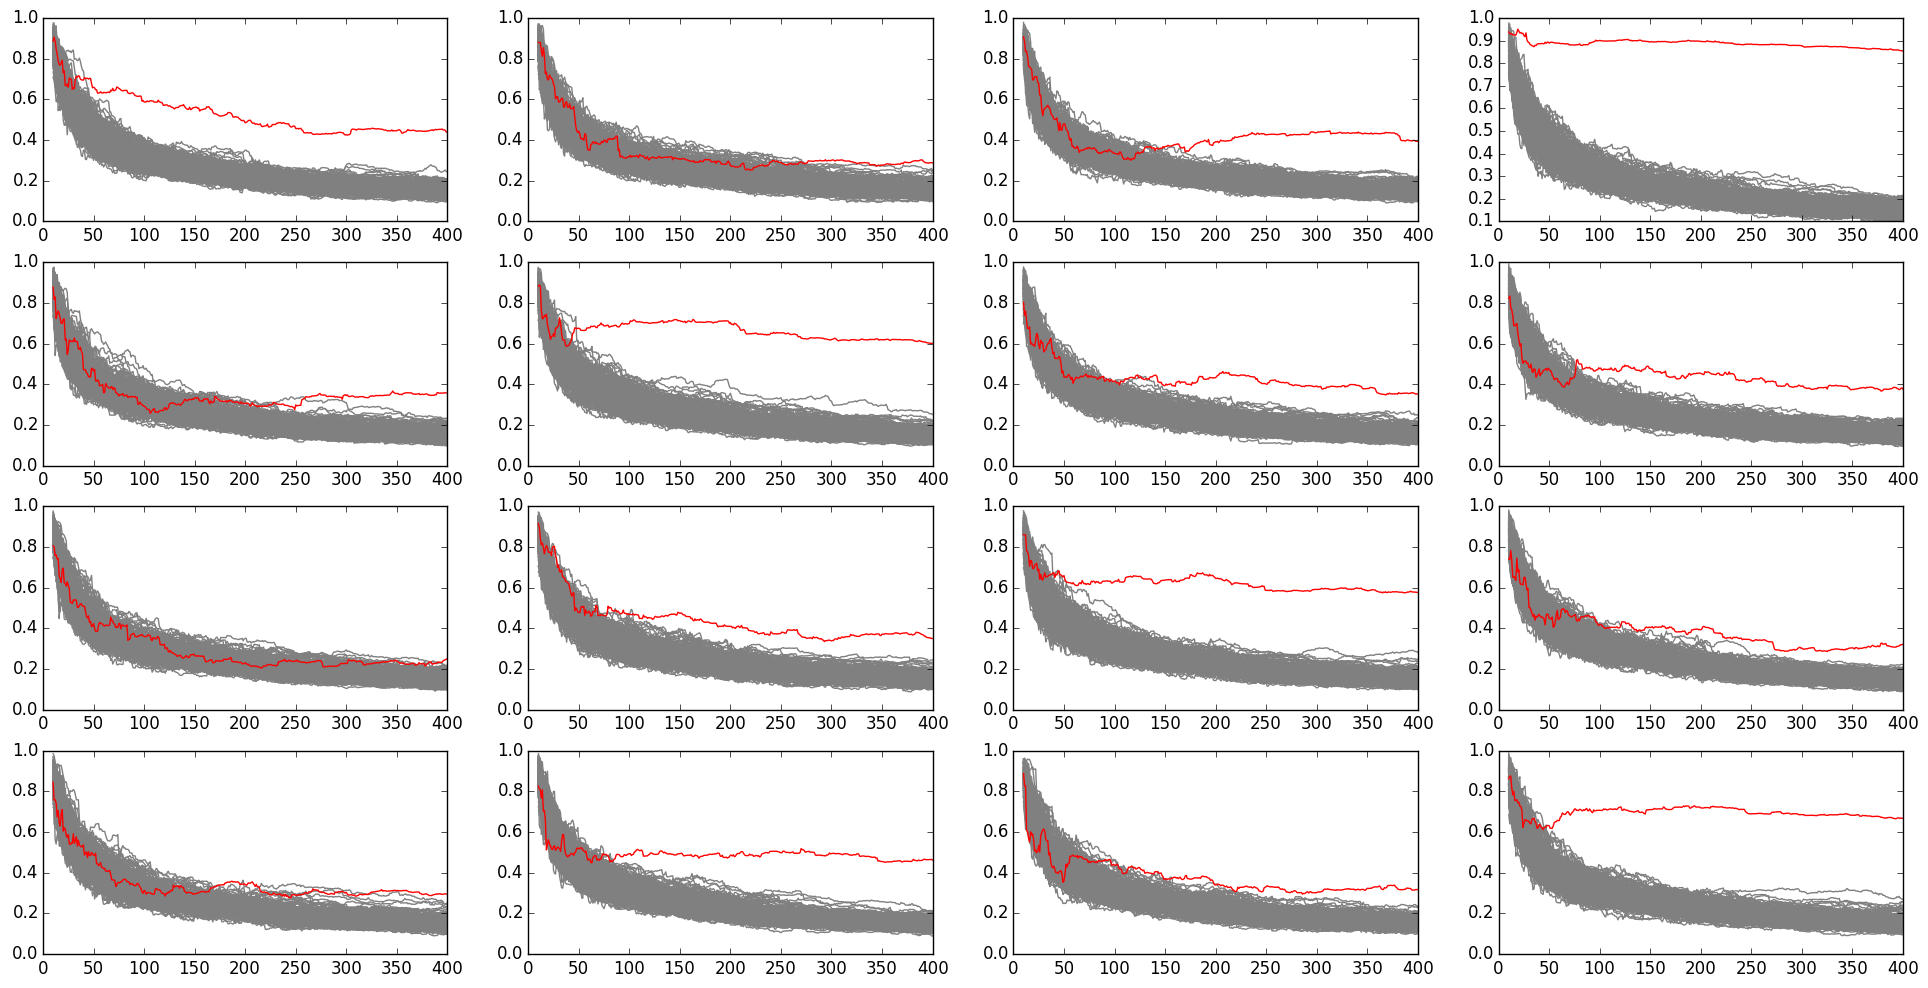
\includegraphics[width=7in]{12-04-15-19-46-23-newrandomkey2-corr-evolution}
\caption{Each graph corresponds to one of the 16 blocks/16 plaintext bytes/16 key bytes in our AES implementation. A single graph plots the correlation of all 256 key guesses (y-axis) with the power trace data, as more data is fed into the correlation (x-axis). The red line represents the correct key guess. Notice that by the time we feed the 400th trace into our CPA implementation, the correct key byte is the key guess with the highest correlation with all the traces (visible in the height of each red line at $x=400$). Results for the other two CPA runs be found Dropbox linked below.}
\label{results_random2}
\end{figure*}

It takes roughly 30 minutes for our infrastructure to collect the traces for the encryption of 100 plaintexts. Data collection time seems to scale linearly with the number of plaintexts we process: iencrypting and collecting the traces for 500 traces, takes on average two and half hours. Processing these 500 traces, and extracting the correlation values and key estimates over $i$ plaintexts for all $i$ (Fig. \ref{results_random2}) takes roughly five minutes.

Our data and results can be found at \texttt{\url{https://www.dropbox.com/sh/07xni6s4tu4klme/AABnrBK-QZCVO1tMK4GFeQ5ta?dl=0}}.

\section*{Acknowledgment}
The authors would like to extend our deepest thanks to Chiraag Juvekar of the Energy Efficient Digital Circuits and Systems group for the time he spent with us aiding our debugging of data collection and analysis problems. We would also like to thank Albert Kwon, our TA, for his insightful advice over the course of the project.


\begin{thebibliography}{1}
\bibitem{ssl}
Lee, Homin K and Malkin, Tal and Nahum, Erich, \emph{Cryptographic strength of ssl/tls servers: current and recent practices}.\hskip 1em plus
  0.5em minus 0.4em\relax Proceedings of the 7th ACM SIGCOMM conference on Internet measurement, 2007.

\bibitem{kerberos}
Rathore, Romendrapal Singh and Pal, BL and Kumar, Shiv. \emph{Analysis and Improvement in Kerberos 5}.\hskip 1em plus
  0.5em minus 0.4em\relax 2015.

\bibitem{embedded}
Altera Corporation, \emph{FPGAs with built-in AES: The key to secure system designs}.\hskip 1em plus
  0.5em minus 0.4em\relax Embedded Computing Design, July 15, 2008.

\bibitem{smalldevice}
Oswald, Elisabeth, et al.  \emph{Side-Channel Analysis Resistant Description of the AES S-Box}.\hskip 1em plus 
  0.5em minus 0.4em\relax 2005.

\bibitem{AESLib}
    \url{https://github.com/DavyLandman/AESLib}. \emph{Arduino AESLib}. \hskip 1em plus
    0.5em minus 0.4em\relax 2015.

\bibitem{daslabor}
    \url{http://www.das-labor.org/wiki/AVR-Crypto-Lib/en}. \emph{AVR-Crypto-Lib}. \hskip 1em plus
    0.5em minus 0.4em\relax 2013.

\bibitem{atmeldatasheet}
    \url{http://goo.gl/hhZF2z}. \emph{Atmel 8-bit Microcontroller Datasheet}. \hskip 1em plus
    0.5em minus 0.4em\relax 2014.

\bibitem{nandflash}
    Handy, Jim. \url{http://goo.gl/5QZHhK} \emph{3D NAND: Making a Vertical String}. \hskip 1em plus
    0.5em minus 0.4em\relax 2013.
\end{thebibliography}
\end{document}


